\subsection{Missing data}
\label{subsec:data-gaps}

\newcommand{\absentPerc}{75.9}
\newcommand{\absentEngPerc}{47.3}
\newcommand{\absentEngOneKPerc}{23.8}
\newcommand{\gapsPerc}{82.2}
\newcommand{\pregapsPerc}{78.0}
\newcommand{\midgapsPerc}{8.0}
\newcommand{\postgapsPerc}{14.1}

\newcommand{\midgapsPossPerc}{32.0}
\newcommand{\midgapsDomainsPerc}{55.0}
\newcommand{\lifespanNoGaps}{11.2}
\newcommand{\lifespanGaps}{16.8}

\newcommand{\numpresentdoms}{130,620}
\newcommand{\numabsentenglishdoms}{150,192}
We categorize missing data into the following categories. For a missing snapshot, we categorize the missing data as follows (also illustrated in figure \ref{fig:missing_types}):
\begin{itemize}
    \item ``absent'': We have no privacy policies on any interval for that website.
    \item ``gap'': We do not have a privacy policy for that snapshot, but we do for a different interval for the same website
    \begin{itemize}
        \item ``pre-gaps'': We do not have a privacy policy for a prior interval, but we do for a later interval
        \item ``mid-gaps'': We have a privacy policy for a prior and a later interval.
        \item ``post-gaps'': We have a privacy policy for a prior interval, but not for a later interval
    \end{itemize}
\end{itemize}


\begin{figure}[t]
\centering
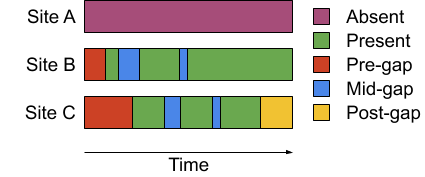
\includegraphics[width=1\columnwidth]{figures/gaps_diagram.png}
\caption{An illustration of the 4 types of missing data. Here we have 3 sites: Site A never appears in our dataset; Site B's first snapshot appears early and has some missing snapshots; Site C's first snapshot appears later, it has some missing snapshots, and has missing snapshots after it's last present snapshot}
\label{fig:missing_types}
\end{figure}

Data can be missing for the reasons described in section \ref{subsec:failure-analysis}. It should not be assumed that because we do not have a privacy policy for a website, that no privacy policy exists for that website. For example, the website may not be in English, Internet Archive may not have a crawl for that interval, or the formatting may have been such that our crawler was not able to find the privacy policy.

We find that \absentEngPerc\% of English websites are absent. We are more likely to have a privacy policy for a popular website: \absentEngOneKPerc\% of the English websites that have been in the Alexa Top 1k are absent.

We find that, for non-absent websites, \gapsPerc\% of possible snapshots are a gap. Of these gaps, \pregapsPerc\% are pre-gaps, \midgapsPerc\% are mid-gaps, and \postgapsPerc\% are post-gaps. The large scale of pre-gaps is expected -- after all, most websites have not existed since 1997, and many websites are not archived by Internet Archive, especially before they gain popularity.

Even with perfect archiving, we expect pre-gaps and post-gaps would still be common, as websites come and go. Therefore, we believe mid-gaps to be the most important gaps to consider. If we assume the first and last intervals where we observe a privacy policy are fixed to be present, and any intermediate interval can be missing or present, we find that mid-gaps constitute \midgapsPossPerc\% of possible mid-gaps. We also find that \midgapsDomainsPerc\% of websites have at least one mid-gap. Longer-lived websites are also more likely to have gaps -- websites for which we have no gaps live an average \lifespanNoGaps~intervals, compared to \lifespanGaps~intervals for websites with gaps.

A mid-gap likely reflects a failure in collection rather than a lack of existence, and mid-gaps are quite common. We therefore recommend that users of the dataset consider imputing mid-gaps with a policy from a preceding or succeeding interval on the same website. The choice of which interval to draw from, and if imputation is needed, depends on the particular research question.

{\textbf{Website popularity.}}
In order to identify if Alexa rank has any bias effects on gaps, we correlated Alexa ranking for a potential snapshot with presence or the gap type. Since gaps are defined for a snapshot, we looked up the Alexa rank for the website during the appropriate interval. For potential snapshots for which we did not have a rank, we assumed the Alexa rank is 1,000,001, i.e., just after the Alexa top 1M list ends. We used Spearman's rank correlation for correlation. The results are shown in Table~\ref{tab:alexa_correlations}. We found that pre-gaps were strongly correlated with Alexa rank, post-gaps were modestly correlated, and mid-gaps were uncorrelated. The correlations are nearly identical when we treat presence in Alexa top 1M as a binary variable. The correlations greatly diminish when we remove all potential snapshots not in the top 1M. This suggests that pre-gaps and post-gaps, but especially pre-gaps, are often caused by the site being unpopular at the time of the gap, which leads to the website not being crawled -- either because it is not a priority or because it does not exist. We also see that mid-gaps have little correlation with Alexa rank, suggesting that other effects are to blame for missing data for mid-gaps.

% \begin{table}[t]
%     \centering
% %    \resizebox{\columnwidth}{!}{%
% \begin{tabular}{@{}lccc@{}}
% \toprule
% \textbf{Gap Type} &\textbf{ $\rho_{c}$} &  \textbf{$\rho_{d}$} & \textbf{$\rho_{1m}$} \\
% \midrule
%          Pre-Gap & 0.51 & 0.59 & 0.06 \\
%          Mid-Gap & 0.06 & 0.09 & -.01 \\
%          Post-Gap & 0.27 & 0.32 & 0.06 \\ \bottomrule
% \end{tabular}%
% %}

%     \caption{Correlations of each type of gap with Alexa rank. $\rho_c$ is the correlation where Alexa rank is an integer from $1$ to $1,000,001$, where missing values are imputed to $1,000,001$. $\rho_d$ is the correlation where Alexa rank is a binary variable representing presence in the top 1M. $\rho_{1m}$ is the correlation where Alexa rank is as in $\rho_c$, but potential snapshots not listed in the Alexa Top 1M are excluded.}
%     \label{tab:alexa_correlations}
% \end{table}

\begin{figure}[t]
\centering
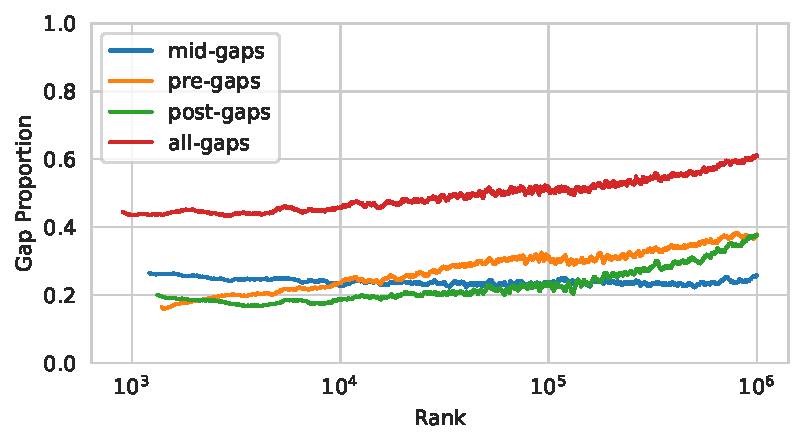
\includegraphics[width=1\columnwidth]{figures/gap_rank_absent.pdf}
\caption{The proportion of snapshots that are gaps as a function of rank. Proportion is calculated as the smooth moving average over the 10,000 neighboring snapshots. Snapshots without a rank are omitted.}
\label{fig:rank_absent}
\end{figure}

\begin{figure*}[t]
\begin{subfigure}[t]{0.45\textwidth}
\centering
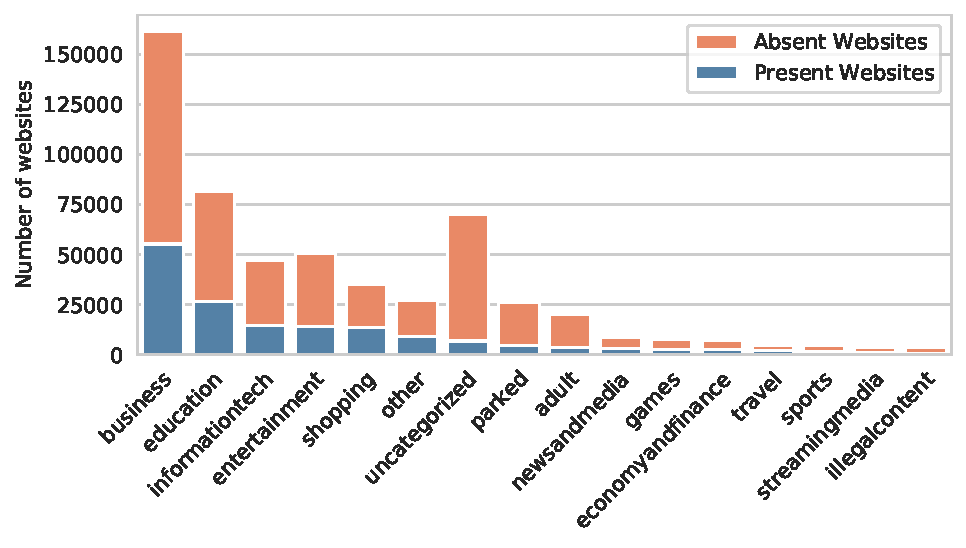
\includegraphics[width=1\columnwidth]{figures/category_dist.pdf}
\caption{The distribution of website categories within our dataset.}
\label{fig:cat_dist}
\end{subfigure}
\hfill
\begin{subfigure}[t]{0.45\textwidth}
\centering
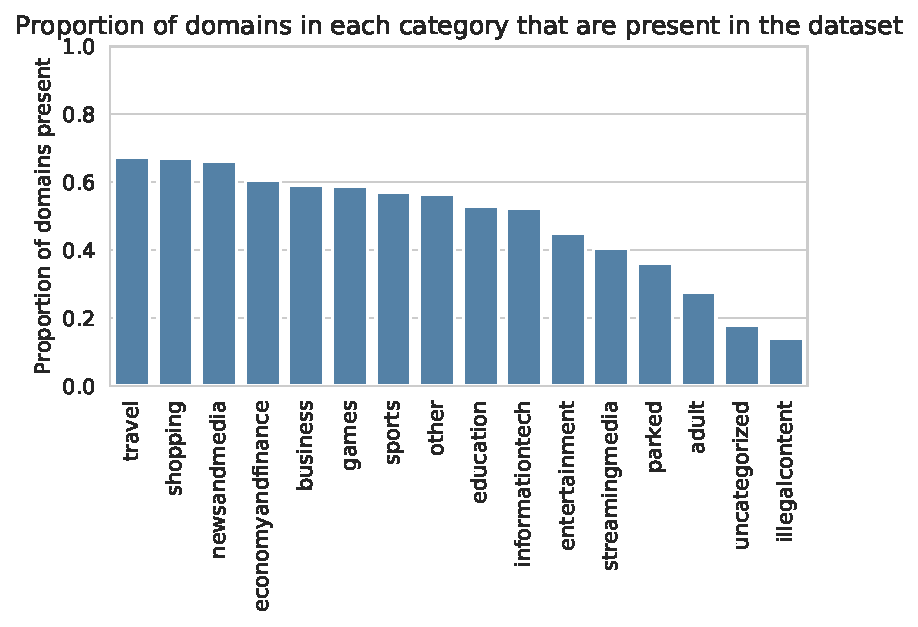
\includegraphics[width=1\columnwidth]{figures/category_missing_perc.pdf}
\caption{The proportion of English-language websites for which we have privacy policies, grouped by category.}
\label{fig:cat_prop}
\end{subfigure}

\caption{The representation of categories in our dataset. ``Other'' is composed of the 27 least frequent categories for English language websites. Policies which belong to multiple categories are counted once per category. Policies with no listed categories are added to the ``uncategorized'' category.}
\label{fig:categories}
\end{figure*}

{\textbf{Distribution of website categories.}}
We further examine the website categories for which we have the best coverage. We collected category data from Webshrinker~\cite{Webshrinker}, which provides a domain category lookup API.
We also collected a small sample of category data from Alexa Web Information Services, but we found the data to be sparse compared to Webshrinker~\cite{awis}; these findings are consistent with those of other researchers~\cite{mathur2019dark}.
Because category data is not available historically from Webshrinker, we made the assumption that categories are constant across time. We collected category data for the \numpresentdoms~websites in our dataset and the \numabsentenglishdoms~websites with English homepages that were at one point in the Alexa Top 100k.
In Figure~\ref{fig:cat_dist} we show the distribution of categories within our dataset. We see that just a few categories dominate most of the dataset.
In Figure~\ref{fig:cat_prop} we show how representative our dataset is of the distribution of English language websites.
We see that for most categories, we capture 40\% or more of the top 100k, English language websites.
However, some categories are strongly
%, though perhaps not unsurprisingly, 
underrepresented in our dataset, such as illegal content\footnote{Illegal content is primarily copyright-infringing content}.